\documentclass[12pt]{article}
\usepackage[utf8]{inputenc}
\usepackage[T2A]{fontenc}
\usepackage[russian]{babel}
\usepackage{amsmath}
\usepackage{amssymb}
\usepackage{geometry}
\usepackage{graphicx}
\usepackage{array}
\geometry{a4paper, margin=2cm}

\begin{document}

\begin{center}
\textbf{Практическое задание к \S8--\S10}\\
\textbf{Вариант 2. Схема Бима--Уорминга}\\[4pt]
Биткулов А., Рыбин Г., Сушков М.
\end{center}


\noindent\textbf{Схема варианта:}
\begin{equation}
y_j^{n+1} = y_j - r(y_j - y_{j-1}) - \frac{r(1-r)}{2}(y_j - 2y_{j-1} + y_{j-2})
\end{equation}

\noindent\textbf{Численный поток:}
\begin{equation}
F_{j+1/2} = a \left( y_j + \frac{1-r}{2}(y_j - y_{j-1}) \right)
\end{equation}

\noindent\textbf{Согласованность потока:}
\begin{equation}
F(y, \dots, y) = a \left( y + \frac{1-r}{2}(y - y) \right) = ay
\end{equation}

\noindent\textbf{Совпадение шага, вычисленного через поток:}
\begin{align*}
y_j^{n+1} &= y_j - \frac{\tau}{h}(F_{j+1/2} - F_{j-1/2}) \\
&= y_j - \frac{\tau}{h} \left[ a \left( y_j + \frac{1-r}{2}(y_j - y_{j-1}) \right) - a \left( y_{j-1} + \frac{1-r}{2}(y_{j-1} - y_{j-2}) \right) \right] \\
&= y_j - r \left[ (y_j - y_{j-1}) + \frac{1-r}{2}(y_j - 2y_{j-1} + y_{j-2}) \right] \\
&= y_j - r(y_j - y_{j-1}) - \frac{r(1-r)}{2}(y_j - 2y_{j-1} + y_{j-2})
\end{align*}

\noindent\textbf{Сохранение:}
\begin{equation}
\sum_j (y_j^{n+1} - y_j)h = -\tau \sum_j (F_{j+1/2} - F_{j-1/2}) = 0
\end{equation}
\textit{(сумма телескопическая, граничные условия периодические)}

\noindent\textbf{2. Ограничитель схемы варианта.}

\noindent Исходная схема:
\begin{equation*}
y_j^{n+1} = y_j - r(y_j - y_{j-1}) - \frac{r(1-r)}{2}(y_j - 2y_{j-1} + y_{j-2})
\end{equation*}

\noindent Поток в форме (10.5) при \(a > 0\):
\begin{equation*}
F_{j+1/2} = a y_j + \frac{a}{2}(1-r)\Delta_{j-1/2}
\end{equation*}

\noindent Функция-ограничитель:
\begin{equation*}
\varphi(\theta) = \theta
\end{equation*}

\noindent Проверка условия (10.6):
\begin{align*}
\theta \le 0 &: \quad \varphi(\theta) = \theta \neq 0 \quad \text{(нарушается)} \\
0 < \theta \le 1 &: \quad 0 \le \theta \le 2\theta \quad \text{(выполняется)} \\
1 < \theta \le 2 &: \quad 0 \le \theta \le 2 \quad \text{(выполняется)} \\
\theta > 2 &: \quad \theta > 2 \quad \text{(нарушается)}
\end{align*}



\bigskip
\noindent\textbf{Уточнение к пункту 2.}
При записи через $\varphi(\theta)$ используется отношение соседних
разностей. Если знаменатель равен нулю, по условию задания полагаем
$\theta=0$. Поэтому именно исходную схему Бима--Уорминга в программе
вычисляем по исходной формуле, а ограниченные схемы --- через поток (10.5).
При ненулевом знаменателе функция исходной схемы равна $\varphi(\theta)=\theta$.

\bigskip
\noindent\textbf{3. Ограничители.}

\noindent Для любого знака $a$ введём $\nu=|a|\tau/h$,
$a^+=\max(a,0)$ и $a^-=\min(a,0)$. В лекции (§10, формула (10.5))
численный поток с ограничителем записан в виде
\begin{equation}
 F_{j+1/2}=a^+y_j+a^-y_{j+1}+
 \frac{|a|}{2}(1-\nu)\varphi(\theta_{j+1/2})(y_{j+1}-y_j).
\end{equation}

\noindent Отношение соседних разностей зависит от знака скорости:
\begin{equation}
 \theta_{j+1/2}=\begin{cases}
 \dfrac{y_j-y_{j-1}}{y_{j+1}-y_j},&a>0,\\[7pt]
 \dfrac{y_{j+2}-y_{j+1}}{y_{j+1}-y_j},&a<0.
 \end{cases}
\end{equation}
Если $y_{j+1}-y_j=0$, принимаем $\theta_{j+1/2}=0$.
При $a=0$ все потоки равны нулю и решение не изменяется.
Новый временной слой находится из консервативной формы:
\begin{equation}
 y_j^{n+1}=y_j^n-\frac{\tau}{h}(F_{j+1/2}-F_{j-1/2}).
\end{equation}

\noindent Четыре ограничителя из определения 10.4:
\begin{align*}
 \varphi_{\mathrm{minmod}}(\theta)&=\max(0,\min(1,\theta)),\\
 \varphi_{\mathrm{vanLeer}}(\theta)&=\frac{\theta+|\theta|}{1+|\theta|},\\
 \varphi_{\mathrm{superbee}}(\theta)&=\max(0,\min(2\theta,1),\min(\theta,2)),\\
 \varphi_{\mathrm{MC}}(\theta)&=\max\left(0,\min\left(2\theta,\frac{1+\theta}{2},2\right)\right).
\end{align*}

\noindent Проверим предельные случаи. При $\varphi=0$ имеем
$F_{j+1/2}=a^+y_j+a^-y_{j+1}$ --- противопоточный поток.
При $\varphi=1$ получаем поток схемы Лакса--Вендроффа:
\begin{equation}
 F_{j+1/2}=\frac{a}{2}(y_j+y_{j+1})-
 \frac{a^2\tau}{2h}(y_{j+1}-y_j).
\end{equation}
В программе оба случая проверены прямым расчётом по этим потокам.

\bigskip
\noindent\textbf{4. Расчёты.}

\noindent Рассматриваем периодическую сетку из $N=200$ ячеек:
\begin{equation}
 h=\frac{1}{N},\qquad x_j=jh,
 \quad j=0,\ldots,N-1.
\end{equation}
Скорость $a=1$, время расчёта $T=1$. Для шагов по времени
берём $\tau=\nu h/|a|$, а последний шаг при необходимости сокращаем,
чтобы получить ровно $T=1$. На последнем шаге пересчитываем $\nu$.
Расчёты проведены при $\nu=0.5$ и $\nu=0.9$.

\noindent Используем начальные профили из файла практики к §§5--6
\texttt{s1-06-practice.py}:
\begin{align*}
 u_0^{\mathrm{step}}(x)&=\begin{cases}0,&0\le x<0.5,\\1,&0.5\le x<1,\end{cases}\\
 u_0^{\mathrm{rect}}(x)&=\begin{cases}1,&0.3\le x\le0.6,\\0,&\text{иначе},\end{cases}\\
 u_0^{\mathrm{gauss}}(x)&=\exp\left(-\frac{(x-0.5)^2}{2\cdot0.05^2}\right),\\
 u_0^{\mathrm{sin}}(x)&=\sin(2\pi x).
\end{align*}

\noindent Точное решение уравнения переноса:
\begin{equation}
 u(x,t)=u_0((x-at)\bmod 1).
\end{equation}
Так как $a=1$ и $T=1$, получаем $u(x,1)=u_0(x)$.
Ошибки и полная вариация вычисляются по формулам
\begin{align*}
 \|e\|_{L_1}&=h\sum_j|y_j-u_0(x_j)|,\\
 \|e\|_C&=\max_j|y_j-u_0(x_j)|,\\
 TV(y)&=\sum_j|y_{j+1}-y_j|.
\end{align*}
Последнее слагаемое $TV$ также учитывает периодический переход
от последней ячейки к первой.

\noindent На каждом шаге проверяем $TV(y^{n+1})\le TV(y^n)+10^{-12}$,
а также сохранение $h\sum_j y_j$.
Для проверки пункта 1 отдельно сравниваем прямую и потоковую реализации
схемы Бима--Уорминга.

\noindent В таблицах ниже приведены итоговые характеристики при $t=1$.
\medskip\noindent\textbf{Ступенька, $\nu=0.5$.}\par\begin{center}\small\begin{tabular}{lrrrrr}\hlineСхема & $L_1$ & $C$ & min $y$ & max $y$ & $TV(y)$\\\hlineБима--Уорминга & 5.232e-02 & 6.111e-01 & -0.2321 & 1.2321 & 3.9470\\Противопоточная & 7.974e-02 & 4.801e-01 & 0.0000 & 1.0000 & 2.0000\\Лакса--Вендроффа & 5.232e-02 & 6.111e-01 & -0.2321 & 1.2321 & 3.9470\\minmod & 3.141e-02 & 4.382e-01 & 0.0000 & 1.0000 & 2.0000\\van Leer & 2.038e-02 & 4.201e-01 & 0.0000 & 1.0000 & 2.0000\\superbee & 8.764e-03 & 3.441e-01 & 0.0000 & 1.0000 & 2.0000\\MC & 1.695e-02 & 4.149e-01 & 0.0000 & 1.0000 & 2.0000\\\hline\end{tabular}\end{center}\medskip\noindent\textbf{Ступенька, $\nu=0.9$.}\par\begin{center}\small\begin{tabular}{lrrrrr}\hlineСхема & $L_1$ & $C$ & min $y$ & max $y$ & $TV(y)$\\\hlineБима--Уорминга & 3.389e-02 & 5.788e-01 & -0.2564 & 1.2564 & 5.4010\\Противопоточная & 3.567e-02 & 4.673e-01 & 0.0000 & 1.0000 & 2.0000\\Лакса--Вендроффа & 2.613e-02 & 5.578e-01 & -0.1640 & 1.1640 & 2.9124\\minmod & 1.787e-02 & 4.120e-01 & 0.0000 & 1.0000 & 2.0000\\van Leer & 1.338e-02 & 4.137e-01 & 0.0000 & 1.0000 & 2.0000\\superbee & 8.121e-03 & 3.445e-01 & 0.0000 & 1.0000 & 2.0000\\MC & 1.170e-02 & 4.000e-01 & 0.0000 & 1.0000 & 2.0000\\\hline\end{tabular}\end{center}\medskip\noindent\textbf{Прямоугольник, $\nu=0.5$.}\par\begin{center}\small\begin{tabular}{lrrrrr}\hlineСхема & $L_1$ & $C$ & min $y$ & max $y$ & $TV(y)$\\\hlineБима--Уорминга & 5.226e-02 & 6.111e-01 & -0.2321 & 1.2321 & 3.9362\\Противопоточная & 7.974e-02 & 4.801e-01 & 0.0000 & 0.9978 & 1.9955\\Лакса--Вендроффа & 5.226e-02 & 6.111e-01 & -0.2321 & 1.2321 & 3.9362\\minmod & 3.141e-02 & 4.382e-01 & 0.0000 & 1.0000 & 2.0000\\van Leer & 2.038e-02 & 4.201e-01 & 0.0000 & 1.0000 & 2.0000\\superbee & 8.764e-03 & 3.441e-01 & 0.0000 & 1.0000 & 2.0000\\MC & 1.695e-02 & 4.149e-01 & 0.0000 & 1.0000 & 2.0000\\\hline\end{tabular}\end{center}\medskip\noindent\textbf{Прямоугольник, $\nu=0.9$.}\par\begin{center}\small\begin{tabular}{lrrrrr}\hlineСхема & $L_1$ & $C$ & min $y$ & max $y$ & $TV(y)$\\\hlineБима--Уорминга & 3.389e-02 & 5.788e-01 & -0.2564 & 1.2564 & 5.4010\\Противопоточная & 3.567e-02 & 4.673e-01 & 0.0000 & 1.0000 & 2.0000\\Лакса--Вендроффа & 2.613e-02 & 5.578e-01 & -0.1640 & 1.1640 & 2.9124\\minmod & 1.787e-02 & 4.120e-01 & 0.0000 & 1.0000 & 2.0000\\van Leer & 1.338e-02 & 4.137e-01 & 0.0000 & 1.0000 & 2.0000\\superbee & 8.121e-03 & 3.445e-01 & 0.0000 & 1.0000 & 2.0000\\MC & 1.170e-02 & 4.000e-01 & 0.0000 & 1.0000 & 2.0000\\\hline\end{tabular}\end{center}\medskip\noindent\textbf{Гауссиан, $\nu=0.5$.}\par\begin{center}\small\begin{tabular}{lrrrrr}\hlineСхема & $L_1$ & $C$ & min $y$ & max $y$ & $TV(y)$\\\hlineБима--Уорминга & 4.689e-03 & 3.490e-02 & -0.0000 & 0.9952 & 1.9905\\Противопоточная & 4.164e-02 & 2.930e-01 & 0.0000 & 0.7070 & 1.4140\\Лакса--Вендроффа & 4.689e-03 & 3.490e-02 & -0.0000 & 0.9952 & 1.9905\\minmod & 4.905e-03 & 7.575e-02 & 0.0000 & 0.9243 & 1.8485\\van Leer & 1.594e-03 & 3.763e-02 & 0.0000 & 0.9624 & 1.9247\\superbee & 3.306e-03 & 2.286e-02 & 0.0000 & 0.9878 & 1.9756\\MC & 8.147e-04 & 2.358e-02 & 0.0000 & 0.9764 & 1.9528\\\hline\end{tabular}\end{center}\medskip\noindent\textbf{Гауссиан, $\nu=0.9$.}\par\begin{center}\small\begin{tabular}{lrrrrr}\hlineСхема & $L_1$ & $C$ & min $y$ & max $y$ & $TV(y)$\\\hlineБима--Уорминга & 7.012e-04 & 5.121e-03 & 0.0000 & 0.9998 & 1.9996\\Противопоточная & 1.112e-02 & 8.762e-02 & 0.0000 & 0.9124 & 1.8248\\Лакса--Вендроффа & 1.198e-03 & 8.773e-03 & -0.0000 & 0.9985 & 1.9969\\minmod & 1.331e-03 & 2.633e-02 & 0.0000 & 0.9737 & 1.9473\\van Leer & 5.752e-04 & 1.432e-02 & 0.0000 & 0.9858 & 1.9717\\superbee & 1.050e-03 & 1.586e-02 & 0.0000 & 0.9946 & 1.9891\\MC & 4.243e-04 & 9.564e-03 & 0.0000 & 0.9906 & 1.9812\\\hline\end{tabular}\end{center}\medskip\noindent\textbf{Синусоида, $\nu=0.5$.}\par\begin{center}\small\begin{tabular}{lrrrrr}\hlineСхема & $L_1$ & $C$ & min $y$ & max $y$ & $TV(y)$\\\hlineБима--Уорминга & 4.935e-04 & 7.751e-04 & -1.0000 & 1.0000 & 4.0000\\Противопоточная & 3.065e-02 & 4.815e-02 & -0.9518 & 0.9518 & 3.8074\\Лакса--Вендроффа & 4.935e-04 & 7.751e-04 & -1.0000 & 1.0000 & 4.0000\\minmod & 1.252e-03 & 8.563e-03 & -0.9914 & 0.9914 & 3.9657\\van Leer & 3.306e-04 & 3.828e-03 & -0.9962 & 0.9962 & 3.9847\\superbee & 9.352e-04 & 5.736e-03 & -0.9991 & 0.9991 & 3.9964\\MC & 1.489e-04 & 2.238e-03 & -0.9978 & 0.9978 & 3.9910\\\hline\end{tabular}\end{center}\medskip\noindent\textbf{Синусоида, $\nu=0.9$.}\par\begin{center}\small\begin{tabular}{lrrrrr}\hlineСхема & $L_1$ & $C$ & min $y$ & max $y$ & $TV(y)$\\\hlineБима--Уорминга & 7.325e-05 & 1.151e-04 & -1.0000 & 1.0000 & 4.0000\\Противопоточная & 6.296e-03 & 9.889e-03 & -0.9901 & 0.9901 & 3.9604\\Лакса--Вендроффа & 1.255e-04 & 1.971e-04 & -1.0000 & 1.0000 & 4.0000\\minmod & 2.531e-04 & 2.731e-03 & -0.9973 & 0.9973 & 3.9891\\van Leer & 1.043e-04 & 1.423e-03 & -0.9986 & 0.9986 & 3.9944\\superbee & 2.035e-04 & 2.500e-03 & -0.9995 & 0.9995 & 3.9980\\MC & 7.194e-05 & 9.233e-04 & -0.9991 & 0.9991 & 3.9964\\\hline\end{tabular}\end{center}
\noindent\textbf{Проверки.} Максимальная разность значений одного шага
между прямой и потоковой формулами Бима--Уорминга составила
$4.44\cdot10^{-16}$, максимальное отклонение дискретной массы
от начальной --- $2.22\cdot10^{-16}$.
Таким образом, сохранение и совпадение формул подтверждены
с точностью машинных вычислений.
Для всех четырёх ограничителей и противопоточной схемы
увеличений TV сверх $10^{-12}$ не обнаружено.
У схем Бима--Уорминга и Лакса--Вендроффа такие увеличения есть.

\noindent Результат для отрицательной скорости дополнительно проверен
на прямоугольнике при $a=-1$, $\nu=0.5$, $N=200$, $t=1$:
масса сохраняется с погрешностью не более $1.67\cdot10^{-16}$;
TVD-ограничители также не увеличивают TV сверх допуска.

\noindent\textbf{Графики.}
Пунктиром отмечено точное решение. Слева показаны исходные схемы,
справа --- четыре ограничителя.
\begin{center}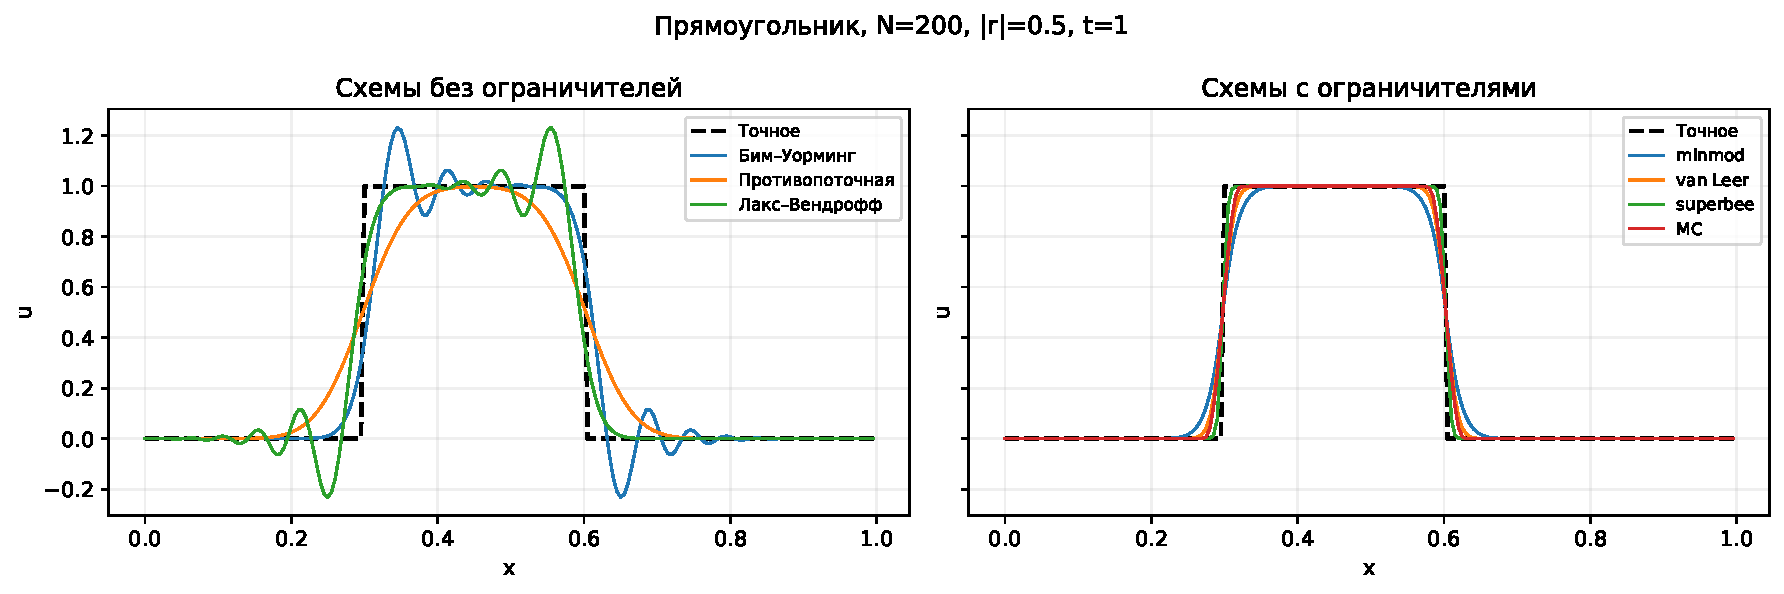
\includegraphics[width=0.96\textwidth]{figures/rectangle_r05.pdf}\end{center}\noindent\textit{Прямоугольник, $\nu=0.5$, $t=1$.}\par\begin{center}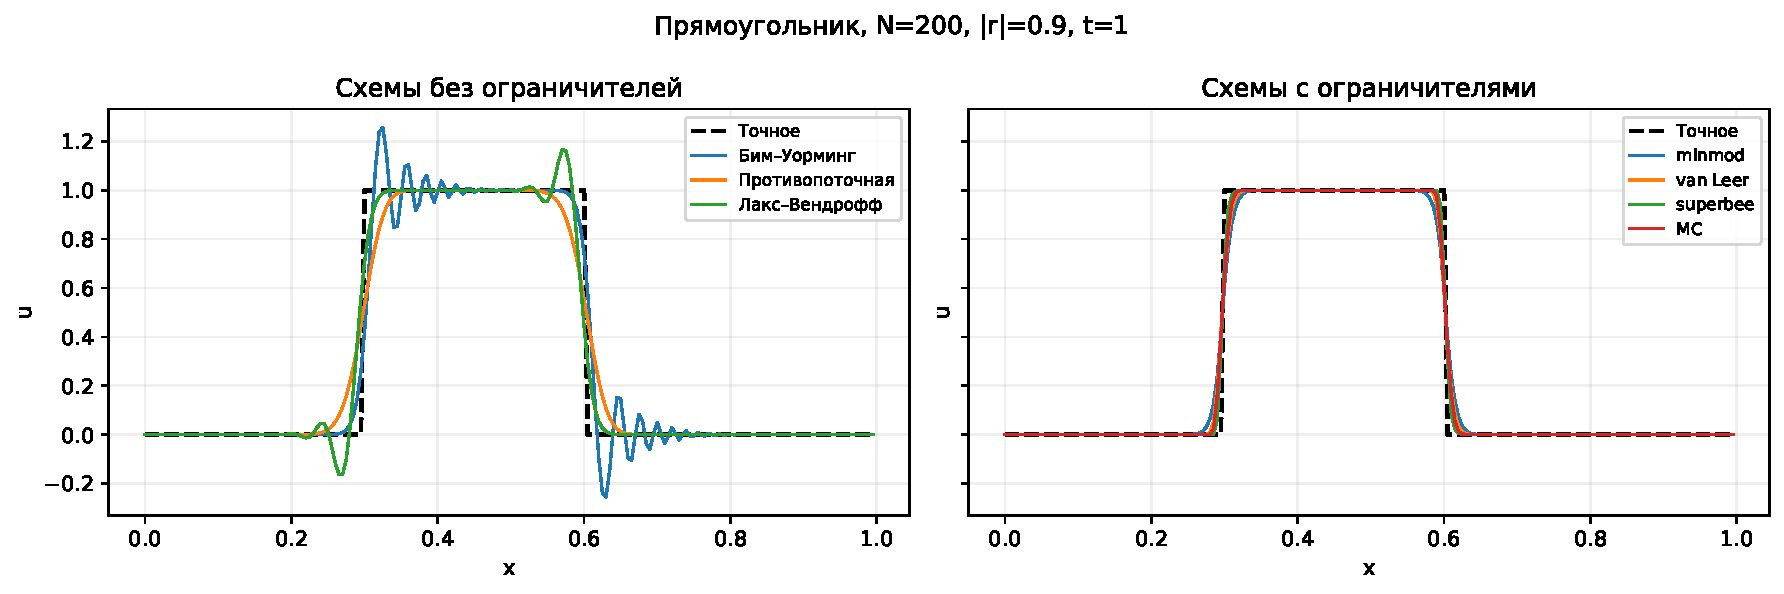
\includegraphics[width=0.96\textwidth]{figures/rectangle_r09.pdf}\end{center}\noindent\textit{Прямоугольник, $\nu=0.9$, $t=1$.}\par\begin{center}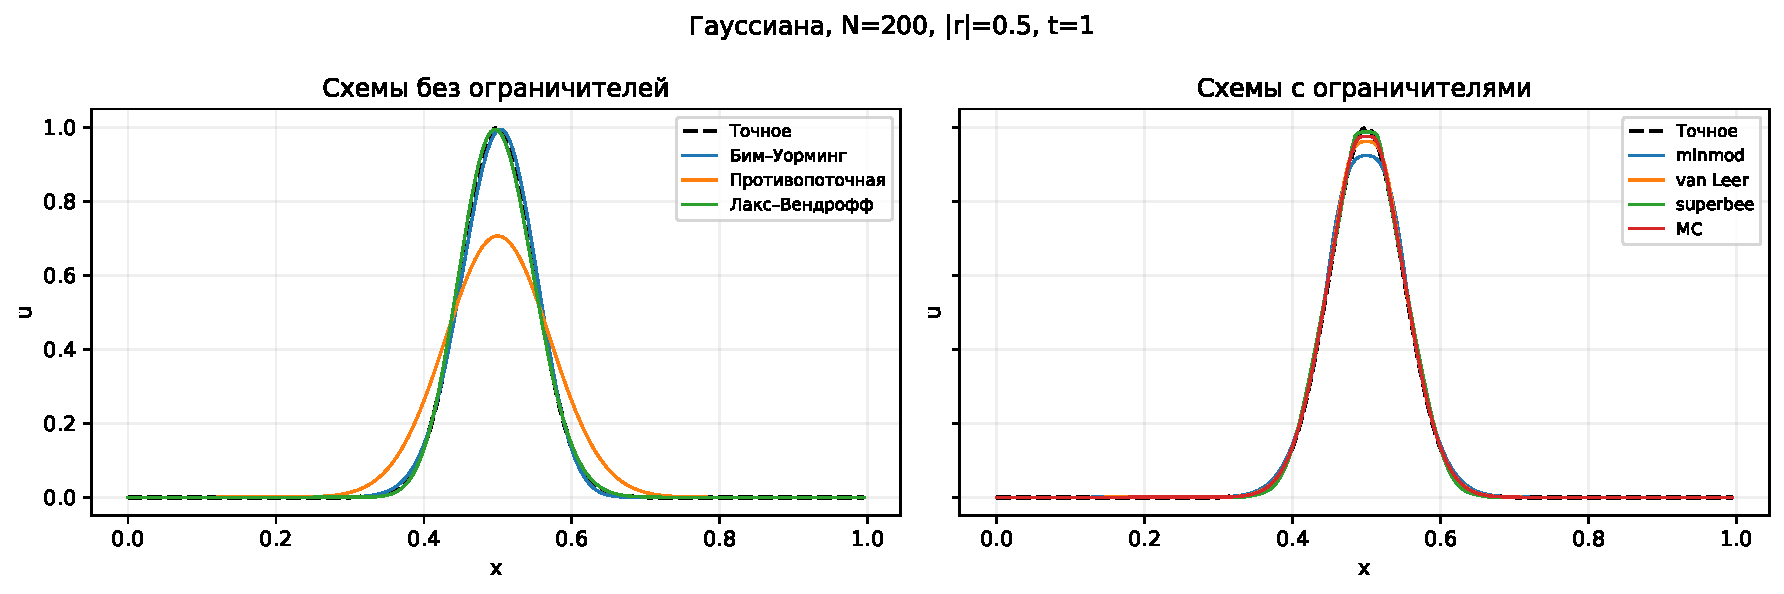
\includegraphics[width=0.96\textwidth]{figures/gaussian_r05.pdf}\end{center}\noindent\textit{Гауссиан, $\nu=0.5$, $t=1$.}\par\begin{center}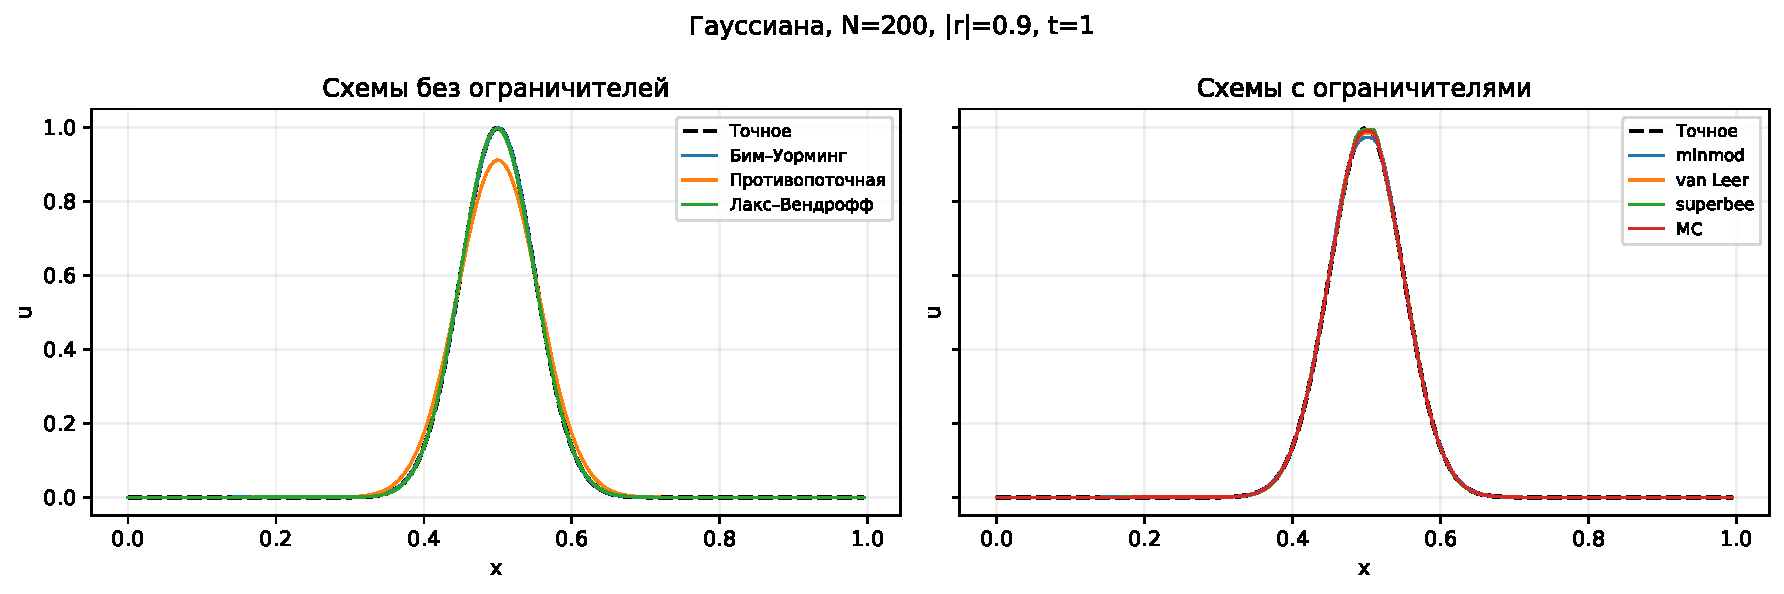
\includegraphics[width=0.96\textwidth]{figures/gaussian_r09.pdf}\end{center}\noindent\textit{Гауссиан, $\nu=0.9$, $t=1$.}\par
\noindent\textbf{Вывод по пункту 4.}
Противопоточная схема не даёт новых экстремумов, но заметно сглаживает
разрывы. Схемы Бима--Уорминга и Лакса--Вендроффа дают колебания
и могут выходить за исходный диапазон значений.
Четыре ограничителя подавляют эти колебания.
На прямоугольнике superbee обычно сохраняет более резкие границы,
а minmod даёт более сильное сглаживание. Эти различия видны и по
ошибкам $L_1$ в таблицах.

\bigskip
\noindent\textbf{5. Наблюдаемый порядок сходимости.}

\noindent Рассматриваем синусоиду на сетках $N=50,100,200,400,800$.
Для всех сеток начальное число Куранта одинаково: $\nu=0.5$.
Порядок вычисляем отдельно в нормах $L_1$ и $C$:
\begin{equation}
 p=\log_2\left(\frac{E_N}{E_{2N}}\right).
\end{equation}
\medskip\noindent\textbf{Схема Бима--Уорминга.}\par\begin{center}\small\begin{tabular}{rrrrr}\hline$N$ & $L_1$ & $C$ & $p_{L_1}$ & $p_C$\\\hline50 & 7.8805e-03 & 1.2371e-02 & --- & ---\\100 & 1.9737e-03 & 3.0989e-03 & 1.997 & 1.997\\200 & 4.9347e-04 & 7.7505e-04 & 2.000 & 1.999\\400 & 1.2337e-04 & 1.9378e-04 & 2.000 & 2.000\\800 & 3.0842e-05 & 4.8447e-05 & 2.000 & 2.000\\\hline\end{tabular}\end{center}\begin{center}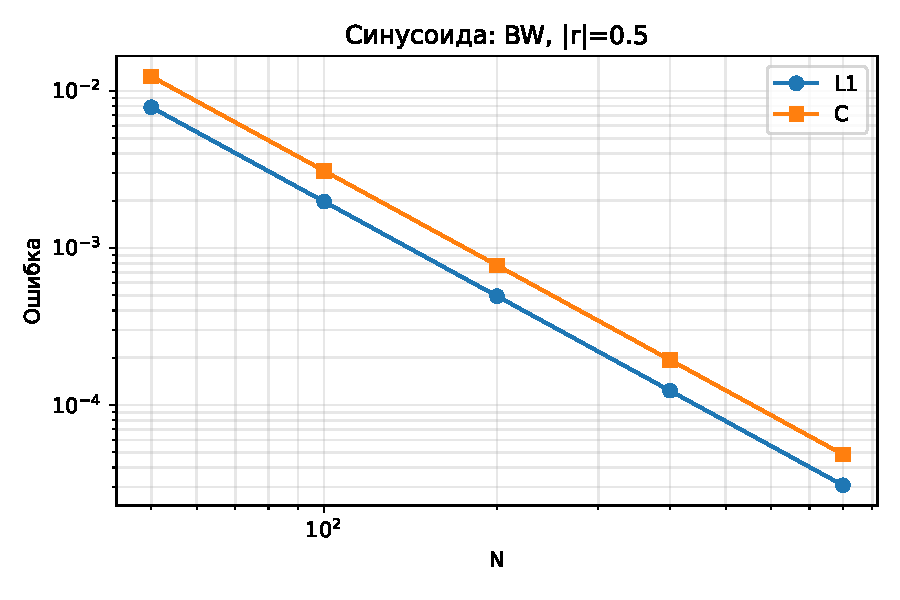
\includegraphics[width=0.65\textwidth]{figures/order_BW.pdf}\end{center}\medskip\noindent\textbf{Схема minmod.}\par\begin{center}\small\begin{tabular}{rrrrr}\hline$N$ & $L_1$ & $C$ & $p_{L_1}$ & $p_C$\\\hline50 & 1.6270e-02 & 4.8986e-02 & --- & ---\\100 & 4.5462e-03 & 2.0981e-02 & 1.839 & 1.223\\200 & 1.2520e-03 & 8.5632e-03 & 1.860 & 1.293\\400 & 3.3696e-04 & 3.4654e-03 & 1.894 & 1.305\\800 & 8.9030e-05 & 1.3953e-03 & 1.920 & 1.312\\\hline\end{tabular}\end{center}\begin{center}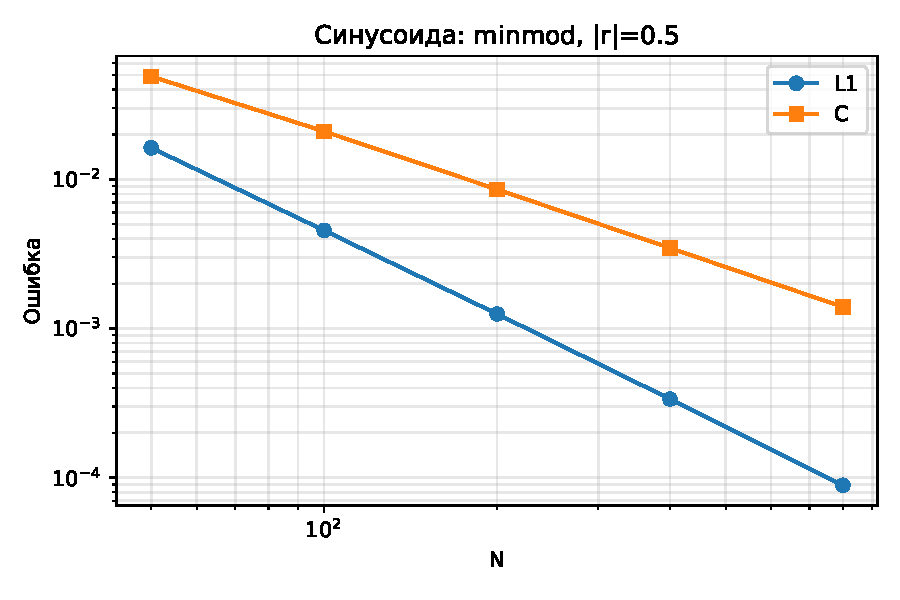
\includegraphics[width=0.65\textwidth]{figures/order_minmod.pdf}\end{center}\medskip\noindent\textbf{Схема van Leer.}\par\begin{center}\small\begin{tabular}{rrrrr}\hline$N$ & $L_1$ & $C$ & $p_{L_1}$ & $p_C$\\\hline50 & 6.1381e-03 & 2.5988e-02 & --- & ---\\100 & 1.4355e-03 & 1.0363e-02 & 2.096 & 1.326\\200 & 3.3061e-04 & 3.8281e-03 & 2.118 & 1.437\\400 & 7.2855e-05 & 1.4031e-03 & 2.182 & 1.448\\800 & 1.5995e-05 & 5.1110e-04 & 2.187 & 1.457\\\hline\end{tabular}\end{center}\begin{center}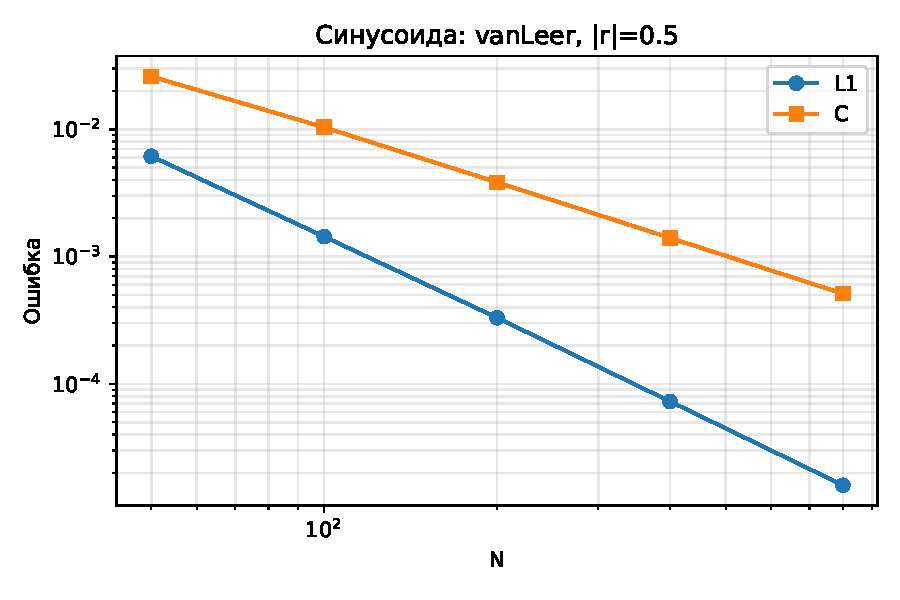
\includegraphics[width=0.65\textwidth]{figures/order_vanLeer.pdf}\end{center}
\noindent\textbf{Вывод по пункту 5.}
У схемы Бима--Уорминга порядок близок к двум в обеих нормах.
У minmod наблюдаемый порядок в $C$ составляет примерно $1.3$,
а в $L_1$ приближается к двум. Для van Leer порядок в $C$
около $1.4$--$1.5$, а в $L_1$ на данных сетках немного превышает два.
Последнее --- наблюдаемый порядок на выбранных сетках, а не утверждение,
что теоретический порядок схемы выше второго.

\noindent Причина потери второго порядка в максимальной норме:
возле максимума и минимума синусоиды производная меняет знак,
поэтому $\theta\le0$. Тогда ограничитель равен нулю, и локально
используется противопоточный поток первого порядка.
В норме $L_1$ такие точки занимают малую часть области,
поэтому уменьшение общей ошибки может оставаться близким ко второму порядку.

\bigskip
\noindent\textbf{6. По варианту.}

\noindent Для схемы Бима--Уорминга получено $\varphi(\theta)=\theta$.
Если ограничить её снизу нулём, а сверху единицей, получим
\begin{equation}
 \varphi_{\rm minmod}(\theta)=\max(0,\min(1,\theta)).
\end{equation}
Это один из четырёх ограничителей определения 10.4.
Он удовлетворяет условию Свеби (10.6): при $\theta\le0$ равен нулю;
при $0<\theta\le1$ равен $\theta$ и не превышает $2\theta$;
при $\theta>1$ равен единице и не превышает $2$.

\noindent\textit{Уточнение.} Одно только условие (10.6) не определяет
верхнюю границу единственным образом. Если ограничить исходную функцию
максимально широко границами всей области Свеби, получится
$\max(0,\min(\theta,2))$, которая не совпадает ни с одной из четырёх
функций на слайде 24. Выбор верхней границы $1$ даёт minmod.

\bigskip
\noindent\textbf{Общий вывод.}
Схема Бима--Уорминга консервативна и имеет второй порядок на гладких
решениях, но около разрывов может давать осцилляции.
Противопоточная схема не даёт таких осцилляций, однако сильнее
сглаживает профиль. Ограничители потока позволяют получить
консервативные TVD-схемы, которые сохраняют хорошую точность
на гладких участках и уменьшают колебания около разрывов.

\noindent\textbf{Программа.} Расчёты выполнены на Python.
Исходный код приложен отдельно.

\end{document}
